%% Copernicus Publications Manuscript Preparation Template for LaTeX Submissions
%% ---------------------------------

\documentclass[gmd, manuscript]{copernicus}

\usepackage{booktabs}
\usepackage{pdflscape}
\usepackage{pdfpages}

\usepackage{multirow}
\usepackage{makecell}
\graphicspath{{./}}
\newcommand{\num}[1]{#1}
\newsavebox{\benchmarktablebox}
\newcommand{\benchmarktablefont}{\normalsize}
\newcommand{\fitwidth}[1]{%
  \sbox{\benchmarktablebox}{#1}%
  \ifdim\wd\benchmarktablebox>\linewidth
    \resizebox{\linewidth}{!}{\usebox{\benchmarktablebox}}%
  \else
    \usebox{\benchmarktablebox}%
  \fi
}


\newif\ifbenchmarklandscape
\AddToHook{shipout/foreground}{%
  \ifbenchmarklandscape
    \AtPageLowerLeft{%
      \put(\LenToUnit{\dimexpr\paperwidth-1.2cm\relax},\LenToUnit{0.5\paperheight}){\rotatebox{90}{\thepage}}%
    }%
  \fi
}
\newenvironment{benchmarklandscape}{%
  \clearpage
  \benchmarklandscapetrue
  \pagestyle{empty}%
  \begin{landscape}%
}{%
  \end{landscape}%
  \benchmarklandscapefalse
  \pagestyle{plain}%
  \clearpage
}

\emergencystretch=2em

\begin{document}

\title{Spherical-shell Stokes flow benchmark using Underworld3}

\Author[1][gthyagi@gmail.com]{Thyagarajulu}{Gollapalli}
\Author[1]{Underworld}{Team}

\affil[1]{Research School of Earth Sciences, Australian National University, Canberra, ACT, Australia}

\runningtitle{Spherical-shell Stokes benchmark in Underworld3}
\runningauthor{Gollapalli}

\received{}
\pubdiscuss{}
\revised{}
\accepted{}
\published{}

\firstpage{1}

\maketitle

\begin{abstract}
We reproduce the analytical spherical-shell Stokes benchmark of
\citet{thieulot2017} using Underworld3 (UW3). The benchmark describes
three-dimensional incompressible viscous flow in a spherical shell with
tangential velocity on both radial boundaries, radial gravity, and a
power-law radial viscosity. We consider the two reference cases used by
\citet{thieulot2017}: \(m=-1\), for which the viscosity is constant, and
\(m=3\), for which the viscosity varies by a factor of 16 across the shell.
The UW3 calculations use a \(P_2P_1\) Taylor--Hood finite-element
discretisation on successively refined meshes with nominal cell size
\(h=1/8,\ldots,1/128\). Velocity and pressure are evaluated using relative
volume \(L_2\)-norm errors, and radial normal stress is evaluated using
relative boundary \(L_2\)-norm errors on the inner and outer spherical
surfaces. The calculations recover the expected asymptotic behaviour for
smooth Stokes solutions, with approximately third-order velocity convergence
and second-order pressure convergence. Boundary radial normal-stress and
boundary pressure errors also approach second-order convergence at the finest
resolutions. These results verify the UW3 curved-domain Stokes discretisation
and provide a compact spherical-shell test for velocity, pressure, and
boundary-stress post-processing.
\end{abstract}

\introduction

Incompressible Stokes flow in spherical shells is a core numerical problem in
global mantle-convection and planetary-interior modelling. Verification in this
geometry is more demanding than in Cartesian boxes because the discretisation
must handle curved boundaries, a pressure nullspace, spherical-coordinate
forcing, radial viscosity variation, and stress quantities evaluated on
non-planar surfaces.

Analytical benchmarks are useful because they separate discretisation and
implementation errors from differences between numerical codes. The benchmark
of \citet{thieulot2017} provides a closed-form solution for viscous
incompressible flow in a spherical shell. The solution is axisymmetric, has no
normal flow on the inner and outer boundaries, uses a radial power-law
viscosity, and supplies analytical expressions for density, velocity, pressure,
body force, and the stress tensor. It therefore tests the Stokes solve and the
post-processing of stress-derived boundary quantities. Related analytical
solutions and finite-element verification studies in curved shell geometries
have been presented by \citet{kramer2021} and \citet{davies2022}, while
boundary normal stress remains a standard diagnostic in spherical geodynamics
benchmarks \citep{zhong1993,zhong2008,liu2019}.

Here we convert the existing UW3 spherical benchmark report into a concise
Copernicus-style article. The aim is to document the governing equations, the
analytical benchmark structure, the numerical setup, the error metrics, and the
observed convergence of velocity, pressure, and boundary stress using the
existing UW3 figures and tables.

\section{Governing equations and benchmark solution}

The benchmark solves the steady incompressible Stokes equations
\begin{subequations}
\begin{align}
  \nabla \cdot \mathbf{u} &= 0, \\
  \nabla \cdot \boldsymbol{\sigma} + \rho\mathbf{g} &= \mathbf{0},
\end{align}
\end{subequations}
where \(\mathbf{u}\) is velocity, \(\rho\) is density, and
\(\mathbf{g}=-\mathbf{e}_r\) is radial gravity of unit magnitude. The stress is
\begin{equation}
  \boldsymbol{\sigma}
  =
  -p\mathbf{I}
  +
  2\mu(r)\boldsymbol{\varepsilon}(\mathbf{u}),
\end{equation}
with pressure \(p\), viscosity \(\mu\), and strain-rate tensor
\begin{equation}
  \boldsymbol{\varepsilon}(\mathbf{u})
  =
  \frac{1}{2}\left(\nabla\mathbf{u}+\nabla\mathbf{u}^{T}\right).
\end{equation}

Following \citet{thieulot2017}, spherical coordinates
\((r,\theta,\phi)\) are used, with \(\theta\) the polar angle and \(\phi\) the
azimuth. All fields are independent of \(\phi\). The tangential velocity
components are prescribed in the separable form
\begin{subequations}
\begin{align}
  u_\theta(r,\theta) &= f(r)\sin\theta, \\
  u_\phi(r,\theta) &= f(r)\sin\theta,
\end{align}
\end{subequations}
and incompressibility gives the radial velocity
\begin{equation}
  u_r(r,\theta)=g(r)\cos\theta,
  \qquad
  g(r)=-\frac{2}{r^2}\int r f(r)\,dr .
\end{equation}
The boundary condition \(u_r=0\) is imposed on the inner and outer shell
surfaces \(r=R_1\) and \(r=R_2\), so the flow is tangential on both boundaries.
The viscosity is
\begin{equation}
  \mu(r)=\mu_0 r^{m+1},
\end{equation}
where \(m=-1\) gives constant viscosity and \(m=3\) gives the radially varying
case considered here.

The pressure has the form
\begin{equation}
  p(r,\theta)=h(r)\cos\theta,
\end{equation}
where the radial pressure coefficient is
\begin{equation}
  h(r)=\frac{2\mu_0}{r}g(r)
  \quad\text{for }m=-1,
  \qquad
  h(r)=\frac{m+3}{r}\mu(r)g(r)
  \quad\text{for }m\neq -1 .
\end{equation}
For \(m\ne -1\), the radial velocity function is obtained from
\begin{equation}
  f(r)=\alpha r^{-(m+3)}+\beta r,
\end{equation}
with \(\alpha\), \(\beta\), and the integration constant in \(g(r)\) chosen so
that \(g(R_1)=g(R_2)=0\). The \(m=-1\) case has the corresponding logarithmic
radial function given by \citet{thieulot2017}. In both cases the density follows
from the radial Stokes
balance after substituting the analytical velocity, pressure, viscosity, and
gravity fields. This construction yields the closed-form density, velocity,
pressure, body force, and stress tensor used for the UW3 error calculations.

\begin{figure}[H]
    \centering
    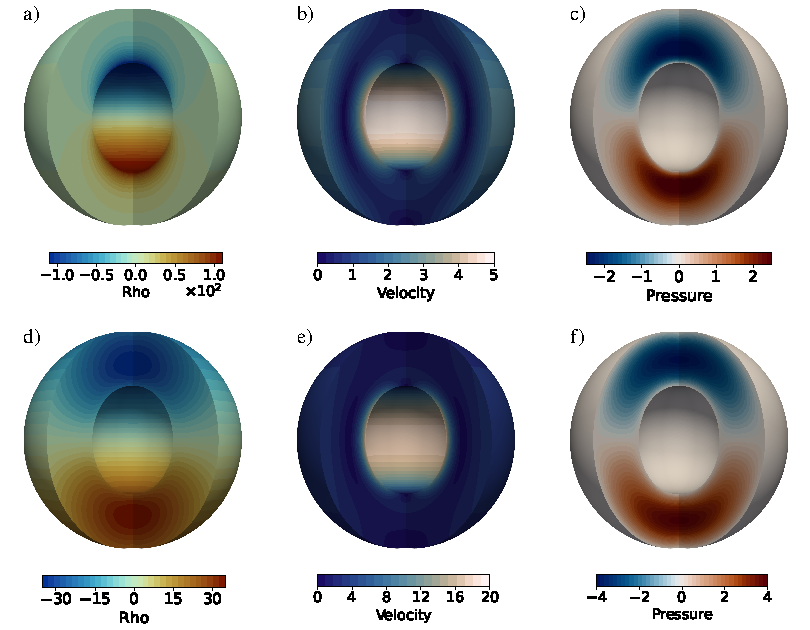
\includegraphics[width=0.92\linewidth]{figure_2_thieulot_analytical.pdf}
    \caption{Analytical density, velocity magnitude, and pressure fields for
    the spherical Thieulot benchmark. The upper row shows the \(m=-1\) case,
    and the lower row shows the \(m=3\) case.}
    \label{fig:thieulot_analytical_fields}
\end{figure}

Figure~\ref{fig:thieulot_analytical_fields} illustrates the analytical fields
used for verification. Both cases satisfy the no-normal-flow condition on the
inner and outer boundaries while retaining non-zero tangential velocity. The
\(m=3\) case uses the same shell geometry but introduces stronger radial
viscosity variation, making pressure and stress recovery more demanding than in
the constant-viscosity case.

\section{Numerical setup}

The benchmark is implemented in UW3 using the finite-element method. The
reported calculations use a \(P_2P_1\) Taylor--Hood element pair, with
quadratic velocity and linear pressure. This pair is expected to give
third-order velocity convergence and second-order pressure convergence in
volume \(L_2\) norms for sufficiently smooth Stokes solutions
\citep{girault1986,boffi2013}. Mesh resolution is reported using the nominal
cell size \(h=1/8,\ldots,1/128\). The analytical velocity is imposed on both
spherical boundaries, and the pressure nullspace is handled by comparing
mean-adjusted numerical and analytical pressure fields.

\section{Error metrics}

For a numerical quantity \(q_h\) and analytical field \(q^*\), the relative
volume error is
\begin{equation}
  E_{L_2}^{\mathrm{rel}}(q)
  =
  \left(
  \frac{\int_\Omega |q_h-q^*|^2\,d\Omega}
       {\int_\Omega |q^*|^2\,d\Omega}
  \right)^{1/2}.
\end{equation}
This metric is used for velocity and pressure. Boundary diagnostics are
evaluated on the inner and outer spherical surfaces, denoted
\(\Gamma_{\mathrm{inner}}\) and \(\Gamma_{\mathrm{outer}}\), using
\begin{equation}
  E_{L_2,\Gamma}^{\mathrm{rel}}(q)
  =
  \left(
  \frac{\int_\Gamma |q_h-q^*|^2\,d\Gamma}
       {\int_\Gamma |q^*|^2\,d\Gamma}
  \right)^{1/2}.
\end{equation}
Absolute boundary pressure errors use the corresponding unnormalised measure
\begin{equation}
  E_{L_2,\Gamma}(p)
  =
  \left(
  \int_\Gamma |p_h-p^*|^2\,d\Gamma
  \right)^{1/2}.
\end{equation}
Observed convergence rates between two consecutive mesh sizes \(h_1\) and
\(h_2\) are computed as
\begin{equation}
  r
  =
  \frac{
    \log\left(E_{h_1}/E_{h_2}\right)
  }{
    \log\left(h_1/h_2\right)
  } .
\end{equation}

\section{Results}

\subsection{Velocity and pressure}

\begin{figure}[H]
    \centering
    
\includegraphics[width=0.98\linewidth]{figures_4_5_thieulot_convergence.pdf}
    \caption{Convergence of the volume \(L_2\)-norm velocity and pressure
    errors for the \(P_2P_1\) discretisation.}
    \label{fig:thieulot_velocity_pressure_convergence}
\end{figure}

\begin{benchmarklandscape}
\begin{table}[p]
\centering
\caption{Spherical Thieulot benchmark convergence for $m=-1$ and $m=3$.}
\label{tab:thieulot_velocity_pressure_rates}
\benchmarktablefont
\setlength{\tabcolsep}{4.7pt}
\fitwidth{%
\begin{tabular}{ccccccccc}
\toprule
\multirow{2}{*}{$h$} &
\multicolumn{4}{c}{$m=-1$} &
\multicolumn{4}{c}{$m=3$} \\
\cmidrule(lr){2-5}
\cmidrule(lr){6-9}
&
$E_{L_2}^{\mathrm{rel}}(\mathbf{u})$ &
\makecell{velocity\\rate} &
$E_{L_2}^{\mathrm{rel}}(p)$ &
\makecell{pressure\\rate} &
$E_{L_2}^{\mathrm{rel}}(\mathbf{u})$ &
\makecell{velocity\\rate} &
$E_{L_2}^{\mathrm{rel}}(p)$ &
\makecell{pressure\\rate} \\
\midrule
$1/8$   & \num{5.842e-03}  & --   & \num{2.287e-01} & --   & \num{3.899e-02}  & --   & \num{3.433e-01} & -- \\
$1/16$  & \num{7.521e-04}  & 2.96 & \num{5.709e-02}  & 2.00 & \num{5.391e-03}  & 2.85 & \num{3.858e-02}  & 3.15 \\
$1/32$  & \num{9.500e-05}  & 2.98 & \num{1.281e-02} & 2.16 & \num{6.630e-04}  & 3.02 & \num{5.959e-03} & 2.69 \\
$1/64$  & \num{1.166e-05} & 3.03 & \num{2.757e-03} & 2.22 & \num{7.628e-05}  & 3.12 & \num{1.179e-03} & 2.34 \\
$1/128$ & \num{1.432e-06} & 3.03 & \num{5.986e-04}  & 2.20 & \num{8.816e-06}  & 3.11 & \num{2.573e-04} & 2.20 \\
\bottomrule
\end{tabular}%
}
\end{table}
\end{benchmarklandscape}

The velocity and pressure errors are shown in
Fig.~\ref{fig:thieulot_velocity_pressure_convergence} and
Table~\ref{tab:thieulot_velocity_pressure_rates}. The velocity error approaches
\(O(h^3)\) for both \(m=-1\) and \(m=3\). The pressure error approaches
\(O(h^2)\) at the finest resolutions, with more irregular coarse-grid rates in
the variable-viscosity case. This behaviour is consistent with the expected
Taylor--Hood convergence hierarchy and with the convergence reported by
\citet{thieulot2017}.

\subsection{Boundary stress and pressure}

\begin{figure}[H]
    \centering
    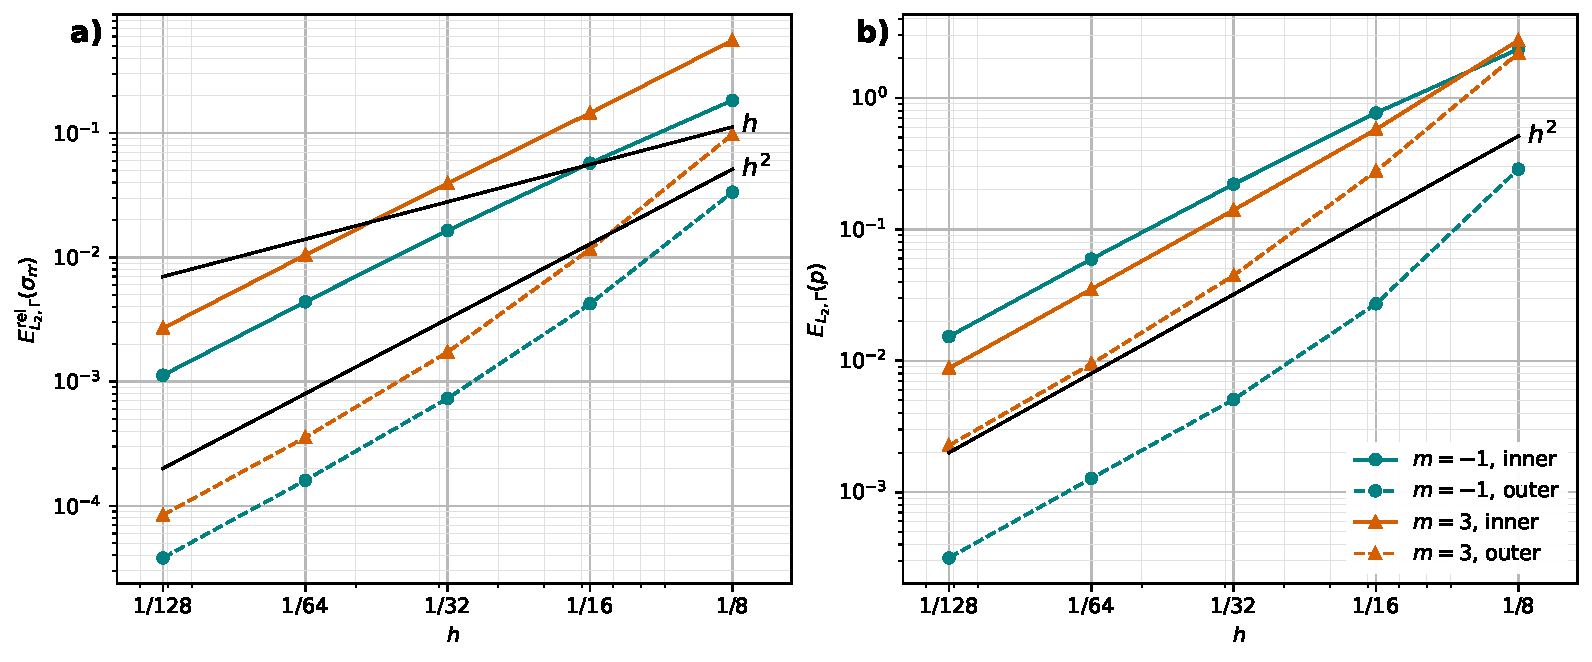
\includegraphics[width=0.98\linewidth]{boundary_metric_convergence.pdf}
    \caption{Convergence of boundary radial normal-stress and pressure errors.
    Solid lines denote the inner boundary and dashed lines denote the outer
    boundary.}
    \label{fig:thieulot_sigma_rr_convergence}
\end{figure}

\begin{benchmarklandscape}
\begin{table}[p]
\centering
\caption{Spherical Thieulot benchmark convergence for boundary $\sigma_{rr}$ errors.}
\label{tab:thieulot_sigma_rr_rates}
\benchmarktablefont
\setlength{\tabcolsep}{4.5pt}
\fitwidth{%
\begin{tabular}{ccccccccc}
\toprule
\multirow{2}{*}{$h$} &
\multicolumn{4}{c}{$m=-1$} &
\multicolumn{4}{c}{$m=3$} \\
\cmidrule(lr){2-5}
\cmidrule(lr){6-9}
&
$E_{L_2,\Gamma_{\mathrm{inner}}}^{\mathrm{rel}}(\sigma_{rr})$ &
\makecell{inner\\rate} &
$E_{L_2,\Gamma_{\mathrm{outer}}}^{\mathrm{rel}}(\sigma_{rr})$ &
\makecell{outer\\rate} &
$E_{L_2,\Gamma_{\mathrm{inner}}}^{\mathrm{rel}}(\sigma_{rr})$ &
\makecell{inner\\rate} &
$E_{L_2,\Gamma_{\mathrm{outer}}}^{\mathrm{rel}}(\sigma_{rr})$ &
\makecell{outer\\rate} \\
\midrule
$1/8$   & \num{1.836e-01} & --   & \num{3.343e-02} & --   & \num{5.578e-01} & --   & \num{9.755e-02} & -- \\
$1/16$  & \num{5.732e-02} & 1.68 & \num{4.233e-03} & 2.98 & \num{1.450e-01} & 1.94 & \num{1.162e-02} & 3.07 \\
$1/32$  & \num{1.644e-02} & 1.80 & \num{7.347e-04} & 2.53 & \num{3.941e-02} & 1.88 & \num{1.730e-03} & 2.75 \\
$1/64$  & \num{4.382e-03} & 1.91 & \num{1.605e-04} & 2.19 & \num{1.044e-02} & 1.92 & \num{3.556e-04} & 2.28 \\
$1/128$ & \num{1.126e-03} & 1.96 & \num{3.811e-05} & 2.07 & \num{2.684e-03} & 1.96 & \num{8.435e-05} & 2.08 \\
\bottomrule
\end{tabular}%
}
\end{table}

\begin{table}[p]
\centering
\caption{Spherical Thieulot benchmark convergence for absolute boundary pressure errors.}
\benchmarktablefont
\setlength{\tabcolsep}{4.5pt}
\fitwidth{%
\begin{tabular}{ccccccccc}
\toprule
\multirow{2}{*}{$h$} &
\multicolumn{4}{c}{$m=-1$} &
\multicolumn{4}{c}{$m=3$} \\
\cmidrule(lr){2-5}
\cmidrule(lr){6-9}
&
$E_{L_2,\Gamma_{\mathrm{inner}}}(p)$ &
\makecell{inner\\rate} &
$E_{L_2,\Gamma_{\mathrm{outer}}}(p)$ &
\makecell{outer\\rate} &
$E_{L_2,\Gamma_{\mathrm{inner}}}(p)$ &
\makecell{inner\\rate} &
$E_{L_2,\Gamma_{\mathrm{outer}}}(p)$ &
\makecell{outer\\rate} \\
\midrule
$1/8$   & \num{2.351e+00} & --   & \num{2.870e-01} & --   & \num{2.739e+00} & --   & \num{2.192e+00} & -- \\
$1/16$  & \num{7.683e-01} & 1.61 & \num{2.712e-02} & 3.40 & \num{5.756e-01} & 2.25 & \num{2.766e-01} & 2.99 \\
$1/32$  & \num{2.206e-01} & 1.80 & \num{5.082e-03} & 2.42 & \num{1.403e-01} & 2.04 & \num{4.455e-02} & 2.63 \\
$1/64$  & \num{5.933e-02} & 1.89 & \num{1.273e-03} & 2.00 & \num{3.505e-02} & 2.00 & \num{9.456e-03} & 2.24 \\
$1/128$ & \num{1.528e-02} & 1.96 & \num{3.162e-04} & 2.01 & \num{8.757e-03} & 2.00 & \num{2.267e-03} & 2.06 \\
\bottomrule
\end{tabular}%
}
\end{table}
\end{benchmarklandscape}

Although \citet{thieulot2017} derive the full stress tensor, the published
benchmark focuses on velocity and pressure convergence. Here the radial normal
stress, \(\sigma_{rr}\), is included as an additional diagnostic because normal
stress on spherical boundaries is important for dynamic-topography and surface
loading calculations. Figure~\ref{fig:thieulot_sigma_rr_convergence} and
Table~\ref{tab:thieulot_sigma_rr_rates} show that \(\sigma_{rr}\) errors
approach approximately second-order convergence on both shell boundaries for
both viscosity cases. The boundary pressure errors show the same asymptotic
trend.

\section{Discussion}

The results verify three aspects of the UW3 spherical-shell Stokes
implementation. First, the \(P_2P_1\) discretisation recovers the theoretical
smooth-solution hierarchy: velocity converges one order faster than pressure in
the \(L_2\) norm. Second, the same rates are obtained for both constant and
radially variable viscosity, although the \(m=3\) case has larger error
constants and stronger pre-asymptotic pressure behaviour. Third, the boundary
radial normal-stress diagnostic converges at roughly second order, consistent
with related spherical-shell stress verification studies \citep{kramer2021}.

The boundary error magnitudes differ between the inner and outer surfaces. This
does not indicate a failure of the benchmark. The relative norms are normalised
separately on two surfaces with different radii, different analytical stress
amplitudes, different curvature, and different local combinations of pressure
and deviatoric-stress error. The verification criterion is therefore the
asymptotic slope, not equality of the error constants.

The benchmark is deliberately compact but still probes several practical issues
for spherical geodynamics solvers: curved boundary representation, pressure
normalisation, radial viscosity variation, tangential velocity boundary
conditions, and stress recovery on spherical surfaces. These properties make it
a useful regression test alongside annulus and Cartesian Stokes benchmarks.

\conclusions

We have presented a Copernicus-style verification article for the UW3
implementation of the Thieulot spherical-shell Stokes benchmark. The benchmark
uses analytical velocity, pressure, density, viscosity, and stress fields in a
curved three-dimensional shell. For the \(P_2P_1\) Taylor--Hood discretisation,
UW3 recovers approximately \(O(h^3)\) velocity convergence and \(O(h^2)\)
pressure convergence for both the \(m=-1\) and \(m=3\) cases. Boundary radial
normal-stress and boundary pressure diagnostics also approach second-order
convergence at the finest resolutions. These results support the use of the
spherical Thieulot benchmark as a production verification case for UW3 velocity,
pressure, and boundary-stress post-processing.

\bibliographystyle{copernicus}
\bibliography{thieulot_spherical_benchmark_article_refs}

\end{document}
